\scanpage{147}
% archive foliation: 146
Soit $C$ une courbe complète, réduite et connexe sur $k$\inserted{alg. clos}.
On veut calculer $\mathrm{Pic}_C$
\diagram{\begin{tikzcd}
0\arrow[r,dash]&\uline{O}_C^*\arrow[r,dash]&\widetilde{\uline{O}}_C^*\arrow[r]&\prod_P A_P^*\arrow[r,dash]&0
\end{tikzcd}\qquad P\ \text{les pts doubles}}
\diagram{\begin{tikzcd}[column sep=small,execute at end picture={
\draw[rounded corners=2pt] ([yshift=-3pt]\tikzcdmatrixname-1-2.south west) -- ++(0,-5pt) -| ([yshift=-3pt]\tikzcdmatrixname-1-4.south east);
\node[below=11pt] at (\tikzcdmatrixname-1-3.south) {$\unsure{G}$};
}]
0\arrow[r]&G_m\arrow[r,dash]&\prod_{C_i}G_m\arrow[r]&\prod_{P_\alpha}A_P\arrow[r]&\mathrm{Pic}_{C/k}\arrow[r]&\prod\mathrm{Pic}_{\widetilde C_i/k}\arrow[r]&0
\end{tikzcd}}
\figure{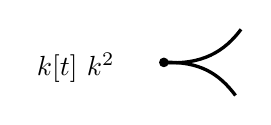
\begin{tikzpicture}[scale=.7]
\node at (-1.6,-.1) {$\unsure{k[t]}\ \unsure{k^2}$};
\fill (0,0) circle (2.5pt);
\draw[very thick] (0,0) .. controls (.7,-.05) and (1.1,.2) .. (1.4,.6);
\draw[very thick] (0,0) .. controls (.65,.02) and (1.0,-.2) .. (1.3,-.6);
\end{tikzpicture}}
On trouve que l'on a dans $\mathrm{Pic}_{\unsure{C^0/k|C/k}}$ une partie linéaire,
\deleted{\unsure{et un gr. multiplicatif}}, qui est isomorphe à
\[
G=\left(\prod_{P_\alpha}A_{P_\alpha}\right)/(\prod G_m/G_m)
\]
donc est de dimension égale à
\[
\dim G=\sum\mu_\alpha-c_0+1
\]
\margin{$c_0=\text{\unsure{nbr des composantes}}\ C_i$}
où $\mu_\alpha=\dim\unsure{A_\alpha|A_{P_\alpha}}$
\deleted{\unsure{\`a}\illegible{2}\ $P_\alpha$} \inserted{$=\dim_k\uline{O}_{\widetilde C}/\uline{O}_C$}.
\unsure{Posons}
\[
\unsure{\mu_\alpha}=1+\delta_\alpha,
\qquad\deleted{\text{\unsure{on trouve donc}}}
\]
\deleted{
\[
\dim G=c_1-c_0+1+\sum\delta_\alpha=b_1+\sum\delta_\alpha
\]
\deleted{\unsure{donc}}
où $b_1$ est le nbr de cycles du schém. combinatoire de $C$.
\margin{$c_0-c_1=1-b_1$}
La dimension de la partie \deleted{multiplicative}\inserted{additive} de $G$ est
\[
\deleted{\unsure{\sum_\alpha(d_\alpha-1)-(\sum d_\alpha)-c_1=2c_0-c_1=}}
\]
\[
\deleted{\unsure{\sum_\alpha(\mu'_\alpha-1)-c_0+1}}
\qquad\sum(\mu_\alpha-\mu'_\alpha)
\]
où $\mu'_\alpha$ est la multiplicité ``ensembliste'' de $P_\alpha$, $=$ nbr de
\deleted{\unsure{courbes}}\inserted{branches formelles} passant par $\alpha$.
}

